\documentclass[10pt]{article}
\usepackage{tikz}
\usetikzlibrary{shapes.misc}
\usepackage[margin=0cm]{geometry}
\pagestyle{empty}
\tikzstyle{every node}=[cross out, draw, red]

\begin{document}

\vspace*{\fill}
\begin{center}
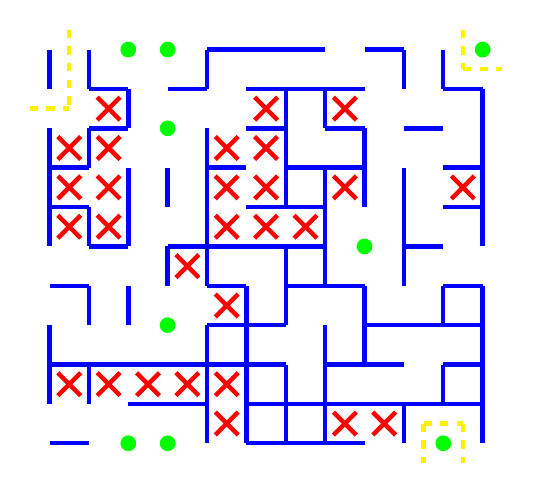
\begin{tikzpicture}[x=0.5cm, y=-0.5cm, ultra thick, blue]
% Walls
    \draw (4,0) -- (7,0);
    \draw (8,0) -- (9,0);
    \draw (1,1) -- (2,1);
    \draw (3,1) -- (4,1);
    \draw (5,1) -- (8,1);
    \draw (10,1) -- (11,1);
    \draw (1,2) -- (2,2);
    \draw (5,2) -- (6,2);
    \draw (7,2) -- (8,2);
    \draw (9,2) -- (10,2);
    \draw (0,3) -- (1,3);
    \draw (4,3) -- (5,3);
    \draw (6,3) -- (8,3);
    \draw (10,3) -- (11,3);
    \draw (0,4) -- (1,4);
    \draw (5,4) -- (7,4);
    \draw (10,4) -- (11,4);
    \draw (1,5) -- (2,5);
    \draw (3,5) -- (7,5);
    \draw (9,5) -- (10,5);
    \draw (0,6) -- (1,6);
    \draw (4,6) -- (5,6);
    \draw (6,6) -- (8,6);
    \draw (10,6) -- (11,6);
    \draw (4,7) -- (6,7);
    \draw (8,7) -- (11,7);
    \draw (0,8) -- (6,8);
    \draw (7,8) -- (9,8);
    \draw (10,8) -- (11,8);
    \draw (2,9) -- (4,9);
    \draw (5,9) -- (11,9);
    \draw (0,10) -- (1,10);
    \draw (5,10) -- (8,10);
    \draw (0,0) -- (0,1);
    \draw (0,2) -- (0,5);
    \draw (0,7) -- (0,9);
    \draw (1,0) -- (1,1);
    \draw (1,2) -- (1,3);
    \draw (1,4) -- (1,5);
    \draw (1,6) -- (1,7);
    \draw (1,8) -- (1,9);
    \draw (2,1) -- (2,2);
    \draw (2,3) -- (2,5);
    \draw (2,6) -- (2,7);
    \draw (3,3) -- (3,4);
    \draw (3,5) -- (3,6);
    \draw (4,0) -- (4,1);
    \draw (4,2) -- (4,6);
    \draw (4,7) -- (4,10);
    \draw (5,6) -- (5,10);
    \draw (6,1) -- (6,4);
    \draw (6,5) -- (6,7);
    \draw (6,8) -- (6,10);
    \draw (7,1) -- (7,2);
    \draw (7,3) -- (7,6);
    \draw (7,7) -- (7,10);
    \draw (8,2) -- (8,4);
    \draw (8,6) -- (8,8);
    \draw (9,0) -- (9,1);
    \draw (9,3) -- (9,6);
    \draw (9,9) -- (9,10);
    \draw (10,0) -- (10,1);
    \draw (10,6) -- (10,7);
    \draw (10,8) -- (10,9);
    \draw (11,1) -- (11,5);
    \draw (11,6) -- (11,10);
% Pillars
    \fill[green] (2,0) circle(0.2);
    \fill[green] (3,0) circle(0.2);
    \fill[green] (11,0) circle(0.2);
    \fill[green] (3,2) circle(0.2);
    \fill[green] (8,5) circle(0.2);
    \fill[green] (3,7) circle(0.2);
    \fill[green] (2,10) circle(0.2);
    \fill[green] (3,10) circle(0.2);
    \fill[green] (10,10) circle(0.2);
% Inner points in accessible cul-de-sacs
    \node at (1.5,1.5) {};
    \node at (5.5,1.5) {};
    \node at (7.5,1.5) {};
    \node at (0.5,2.5) {};
    \node at (1.5,2.5) {};
    \node at (4.5,2.5) {};
    \node at (5.5,2.5) {};
    \node at (0.5,3.5) {};
    \node at (1.5,3.5) {};
    \node at (4.5,3.5) {};
    \node at (5.5,3.5) {};
    \node at (7.5,3.5) {};
    \node at (10.5,3.5) {};
    \node at (0.5,4.5) {};
    \node at (1.5,4.5) {};
    \node at (4.5,4.5) {};
    \node at (5.5,4.5) {};
    \node at (6.5,4.5) {};
    \node at (3.5,5.5) {};
    \node at (4.5,6.5) {};
    \node at (0.5,8.5) {};
    \node at (1.5,8.5) {};
    \node at (2.5,8.5) {};
    \node at (3.5,8.5) {};
    \node at (4.5,8.5) {};
    \node at (4.5,9.5) {};
    \node at (7.5,9.5) {};
    \node at (8.5,9.5) {};
% Entry-exit paths without intersections
    \draw[dashed, yellow] (10.5,0.5) -- (11.5,0.5);
    \draw[dashed, yellow] (-0.5,1.5) -- (0.5,1.5);
    \draw[dashed, yellow] (9.5,9.5) -- (10.5,9.5);
    \draw[dashed, yellow] (0.5,-0.5) -- (0.5,1.5);
    \draw[dashed, yellow] (9.5,9.5) -- (9.5,10.5);
    \draw[dashed, yellow] (10.5,-0.5) -- (10.5,0.5);
    \draw[dashed, yellow] (10.5,9.5) -- (10.5,10.5);
\end{tikzpicture}
\end{center}
\vspace*{\fill}

\end{document}
